\chapter{虚拟试验编著系统的设计与实现}
\label{report}

本系统针对教育者进行开发,因此需要为他们提供一套用户友好的编著系统,使他们可以通过此系统自主创建实验用于教学。本章节将对该系统的用户需求、设计与实现、结果分析进行阐述。

\section{编著系统需求分析}
本系统是面向教育者和学生开发的,因此在需求分析上,主要从他们的角度出发。

\subsection{交互需求}
对于教师来说,他们通常不具有编程能力,因此所有编辑功能都应该封装起来,只留下简单明晰的用户接口。教师往往没有太多时间学习新系统,交互方式应当符合直觉或常识,例如拖动移动物体、点击编辑物体等。此外,对系统不熟悉的人,不熟悉系统的使用流程。一方面,在降低用户的学习成本的同时,应当适当的进行操作指示和辅助。例如在交互界面显示提示字板,或在用户初次使用的时候,对用户进行引导。另一方面,用户在未知的情况下很可能做出很多设想之外的操作,或违规操作,这些操作应当尽可能从代码层面避免。

\subsection{功能需求}
目前的教学辅助应用可以为学生提供个性化和应试两个方面的辅导。在个性化的方面,增强现实应用本身就可以为学生提供更丰富的学习体验,扩展视野。这要求应用在增强现实方面尽可能做到虚实融合效果稳定可靠、视觉效果优良,并且为用户提供丰富而自由的交互。在应试方面,则需要教学辅助应用利用可重复性高的特点,为学生的实验考试提供帮助。例如,在引导学生进行实验的时候,应当关注于用户操作的准确性,包括各种仪器的使用方式、实验流程等。此外,对于错误操作应当进行警告与纠正。还可以模拟一些实验操作的试题,例如在规定产物以及生成量的基础上,由学生自主设置反应药品和反应量等等。

\subsection{硬件平台}
根据实际学校的使用情况,应用的硬件平台也应满足一定的要求。首先,设备本身成本不宜过高,对于一个40人的班级来说,平均需要两人一套设备,这本身就是很大的开销。另外,设备所占场地也应该尽可能小,因为学校的教室、实验室的空间都比较有限。手机交互就是一种比较理想的方式。为了保证手机交互的便捷,应当避免手指难以实现的交互操作,例如鼠标悬停等。此外,电脑作为最广泛被使用的平台,也应当被支持。

\subsection{功能总结}
从编著系统的功能来说,本项目基于化学引擎进行开发,得出需要实现的功能有,用户可以编辑实验环境,如场景灯光颜色和亮度、相机高度和角度等。用户可以添加实验仪器或药品,移动他们的位置、编辑容器所含药品的种类和物质的量等。用户可以修改实验提示信息的颜色、位置、大小。用户可以自主编辑实验流程,包括实验的标题,每一个流程的名称(如预热),每个流程包含的子步骤的名称(如点燃酒精灯)以及对应的事件名称等。事件用于在进行实验的过程中将用户自定义的实验步骤名称与系统中统一的实验操作对应。

\section{编著系统设计}
编著场景为Build Experiment,负责创建、编辑虚拟实验。它基于Unity引擎进行开发,由引擎中的游戏管理器进行管理。其中的架构分为三层。

\begin{figure}[!htp]
  \centering
  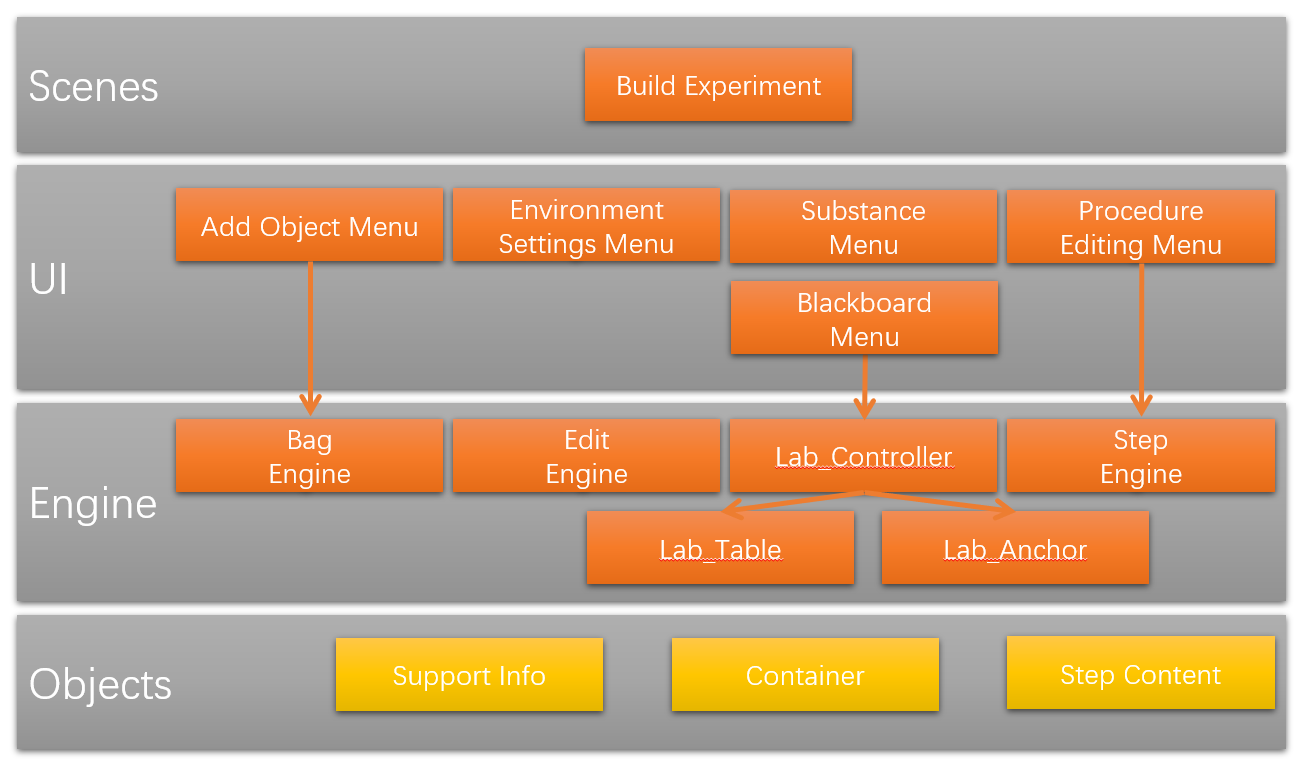
\includegraphics[width=12cm]{figure/buildearc.png}
  \bicaption[编著场景架构设计图]
    {编著场景架构设计图}
    {The Building Experiment Scene Architecture Design}
 \label{fig:gm}
\end{figure}

最上层为用户接口(User Interface,UI),他保存了用户前端的控件。前端控件主要由五个菜单构成。

\begin{itemize}
    \item \textbf{Add Object Menu}
用户可以通过此菜单向场景中添加物体。在菜单中对各类物体进行分类,对于化学实验来说,分为容器、物质、工具、预置组合四类。
    
    \item \textbf{Environment Settings Menu}
用户可以通过此菜单修改实验环境,例如场景的灯光强度与颜色、室内或是室外环境、相机的高度与角度等。
    
    \item \textbf{Blackboard Menu}
用户可以通过此菜单修改实验中的实验操作提示的大小、颜色,包括显示实验标题的文字和显示实验操作的正文两个部分。

    \item \textbf{Substance Menu}
用户可以通过此菜单修改容器所含的的物质的种类及其物质的量。

    \item \textbf{Step Menu}
用户可以通过此菜单修改实验的标题、流程、每个流程包含的子步骤等内容。由于用户的步骤名称是多样的,同一个行为可能有多种表达方式,因此系统还提供了事件选项,用与将用户输入的操作与系统中实际实现和进行判断的操作对应。

\end{itemize}
~\\
\indent    	上述的控件需要第二层——引擎进行支撑。由于编著系统很大程度上集中在UI的部分,因此引擎大部分是为UI服务的。除此以外,应用还具有其他交互形式,也是由引擎实现的。

\begin{itemize}
    \item \textbf{Bag Engine}
用于控制Add Object Menu。其中包括Menu出现和消失的动画、菜单不同类别之间切换的逻辑、获取用户希望添加的物体等功能,并且向更底层的引擎传递用户输入事件。
    
    \item \textbf{Edit Engine}
用于管理编著场景中的所有数据,包括场景中添加物体的位置、种类,容器中的药品的种类与量,实验提示文字的位置、颜色、大小,场景中的环境数据等。引擎会在用户编辑完成的时候将所有数据采用固定的格式进行保存,在编辑已有场景的时候从该数据结构中进行读取并且还原,两者共用同一个场景。
    
    \item \textbf{Step Engine}
用于控制Step Menu。负责用户创建、编辑每个实验对应的标题、流程、步骤等信息。

    \item \textbf{Lab Controller}
是交互的核心控制引擎,获得鼠标(或手指触摸)事件,运行相应的业务逻辑。判断输入的是点击事件还是长按事件,如果是点击事件则弹出编辑界面,包括提示信息的编辑界面(Blackboard Menu)、物质的编辑界面(Substance Menu)两种。如果是拖动事件,则将被点击的物体或文字进行移动。在编辑已有实验的时候,需要从游戏管理器中读取已创建的物质以及黑板信息数据,并且进行还原。在桌面上拖动时,可以选择固定的锚点上,或是锚点范围外的任意位置。设置锚点的目的是可以使一些仪器保持固定的相对位置和顺序,这些锚点本身是Lab Anchor对象,提供在锚点上添加、替换、删除物体等操作。Lab Anchor由Lab Table进行统一维护,包括在用户在锚点内外移动、添加物体的时候控制所有锚点的行为。例如,在用户将物体移入锚点范围的时候,Lab Table会在在指定的锚点中空出位置;在用户将物体从锚点拖离的时候,它会用其他锚点上的物体填补空缺等。

    \item \textbf{Button}
对于场景中一直显示的按钮,如展开环境设置菜单的按钮,展开加入物体菜单的按钮等,都在Button中统一实现了点击事件响应函数。它还控制在有菜单被展开的时候暂停Lab Controller中物体控制的逻辑(物体点击、拖动),避免用户在使用菜单时的操作干扰实验编辑。
\end{itemize}
~\\
\indent    	上述逻辑需要使用一些持久化的对象封装和储存信息,这些对象包括保存用户创建容器所含物质的种类和量的对象Container,保存用户创建的步骤和流程的对象Step Content,保存实验提示信息的颜色和大小信息的text,保存系统支持的物质和时间类型的对象Support Info等。

此外,保存的数据也使用了持久化的对象Experiment Setup进行保存,但属于游戏管理器而非某个场景,其UML类图\ref{fig:uml}如图所示。


\begin{figure}[!htp]
  \centering
  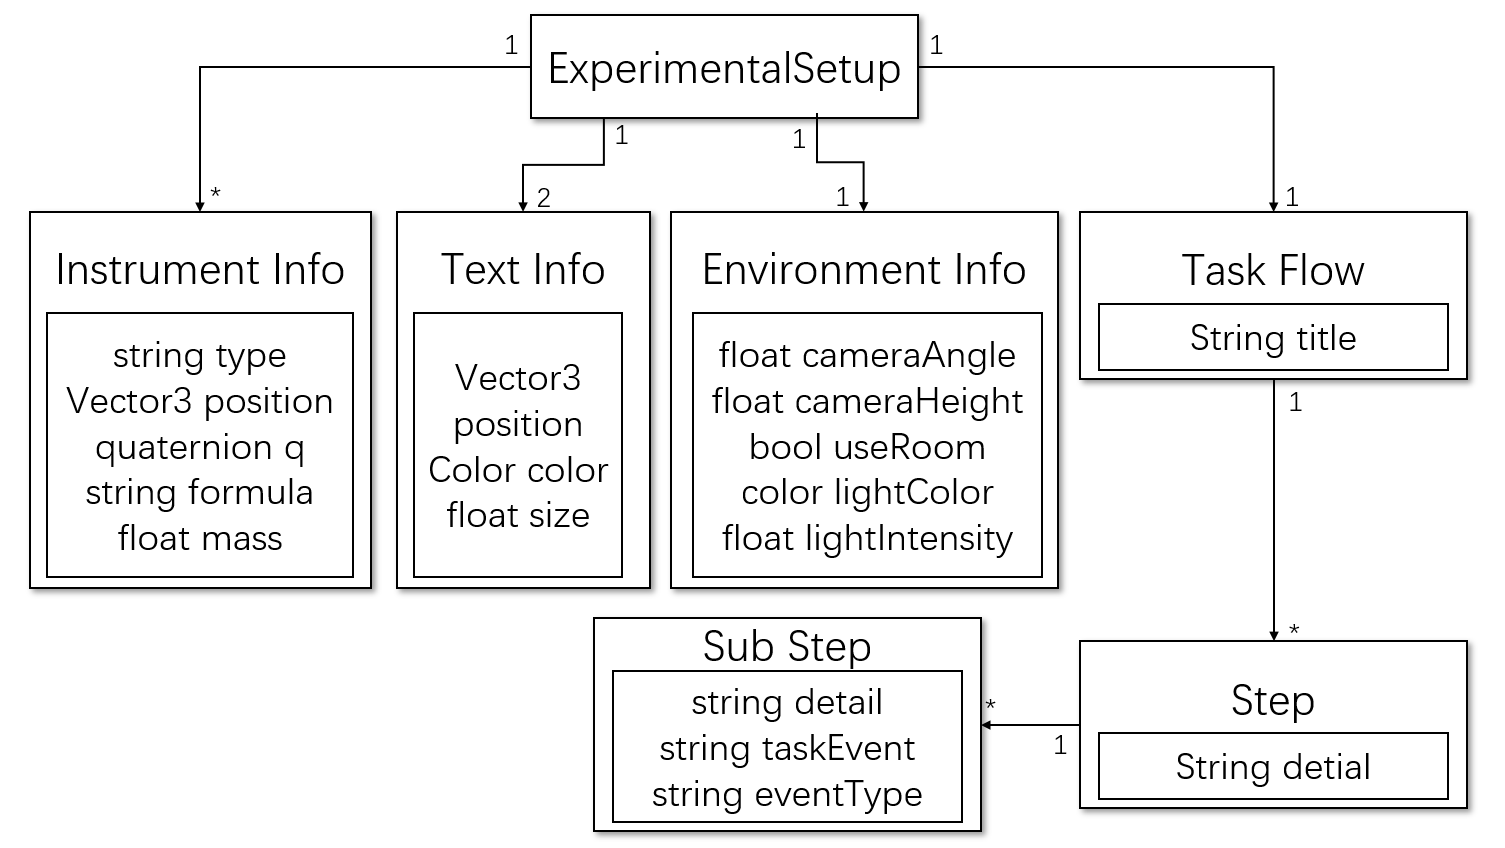
\includegraphics[width=12cm]{figure/setupclass.png}
  \bicaption[编著信息UML类图]
    {编著信息UML类图}
    {The UML's class Diagram of Authored Data}
 \label{fig:uml}
\end{figure}

其中编著信息由四部分组成。每个场景有多个instrument info保存创建的物体的位置、旋转、物体种类、其中含有的物质的名字及其物质的量。每个场景由两个text info,分别用来储存实验提示信息中的标题和正文的位置、大小、颜色信息。每个场景包括一个environment info,用来保存场景中相机、光照的相关属性。每个场景还包括一个task flow,用来保存编辑的实验流程。每个实验流程有多个流程(step),每个流程又有多个步骤(substep),步骤中包含步骤名称、对应的事件等信息。

\section{编著系统的实现}

编著功能主要在Build Experiment场景中进行实现,本小节将首先介绍场景中的用户接口(UI),然后根据需求进行相应的介绍。

\subsection{用户接口(UI)实现}
编著场景中实现了五个用于交互的菜单。

\begin{itemize}
    \item \textbf{Settings Menu}
用于修改实验场景。实验环境编辑需要调整光照颜色与强度,相机高度与角度,实验环境(室内或是室外)等。因此使用了滑块(Slider)和开关(Switch)等控件,并添加一个半透明panel用于和场景区分。滑块封装了OnValueChange函数,会在滑块发生移动的时候触发。相似的,开关控件会在被修改的时候调用控制函数。
    
    \item \textbf{Tool Menu}
用于添加物体。用户点击添加物体按钮后,会播放动画显示选择物体类别的菜单,用户选择要添加的物体类别,之后彩电显示该类别下所有支持物体的图片,用户点击对应图片添加物体。选择物体类别的菜单由UI\_List实现,目前支持“容器”、“药品”、“工具”、“预置组合”四类。UI\_List本身具备垂直布局(vertical layout),将子对象自动按照垂直排列。每一个子对象对应一种物体类别,并且绑定了onclick函数。选择类别后弹出的选择具体物体的菜单由UI\_Bag实现,包含了一个网格布局(grid layout),自动将子对象按照网格排列。他的子对象都是预制体(prefab),可以显示图片,并且绑定了创建物体的onclick函数。
    
    \item \textbf{Substance Menu}
用于编辑容器所含药品及其物质的量。其中包括,选择物质种类的下拉框(dropdown),以及输入物质的量的输入框(input field)。下拉框使用了OnValueChange函数,在选择变化时触发。输入框绑定OnEndEdit函数,在编辑完成时触发。

    \item \textbf{Blackboard Menu}
用于编辑场景中的实验操作提示。包括调整文字的大小和颜色,实现与settings menu类似。
    
    \item \textbf{Step Menu}
用于设置实验的步骤等信息。最上方设置了输入实验名称的输入框。左侧使用了vertical layout显示当前的已有的流程,右侧显示该流程当前已有的步骤。流程和步骤都使用了同一个预置体。中间提供了输入流程名称、步骤名称的输入框,以及选择对应事件的下拉框。他们都绑定了对应的OnValueChange函数,在获得用户输入的时候触发。
\end{itemize}
~\\
\indent    	上述菜单会通过场景中的按钮或用户输入触发,同时会暂停触发场景其他交互行为,防止在用户调整菜单的时候干扰。在菜单之下还会生成一个覆盖整个屏幕的透明按钮,实现当用户点击的时候关闭菜单,并且确定用户输入,恢复场景其他交互。

\subsection{实验场景编辑}
当用户点击场景编辑按钮后,会弹出编辑场景的菜单(Settings Menu)。用户移动其中的滑块时,会触发OnValueChange函数,调用控制Slider的引擎,UI\_Slider,它保存了场景中相机、光源的指针,会读取此时slider的值,并且修改对应对象的属性值。如果通过开关调整实验环境,开关的控制器会修改对应的场景模型。

\begin{figure}[!htp]
  \centering
  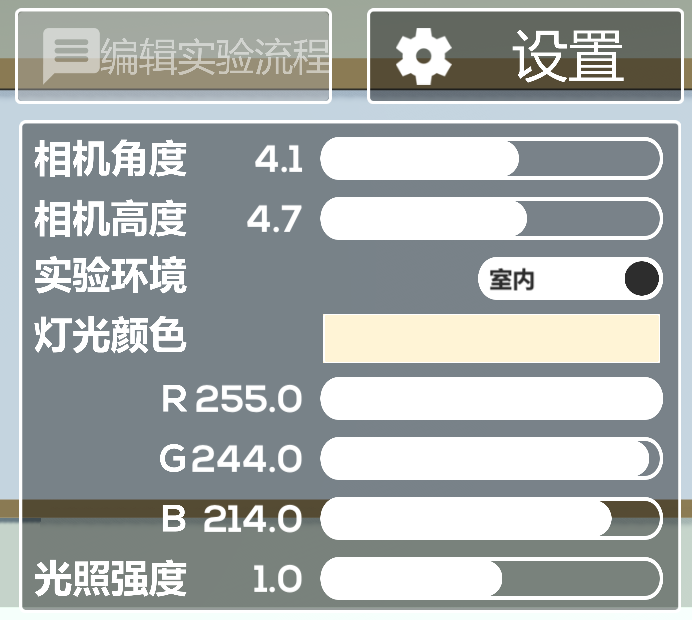
\includegraphics[width=8cm]{figure/settings.png}
  \bicaption[实验场景编辑用户接口截图]
    {实验场景编辑用户接口截图}
    {The Screen-shot of Experiment Editing UI}
 \label{fig:gm}
\end{figure}

\subsection{物体编辑}
场景中的物体通过菜单进行添加。支持物体以及他们的种类通过静态二维链表储存。

	当用户选择添加物体之后,选择物体种类的菜单弹出(Tool Menu)。物体种类被选择后,控制器UI\_List会查找二维链表,获得对应类别的物体图片,并创建显示该图片的预制体,添加到选择物体的菜单中。用户选择物体之后,会通过物体的名字,在资源文件夹中查找对应的预制体游戏对象,添加到场景中,完成物体创建。
	
\begin{figure}[!htp]
  \centering
  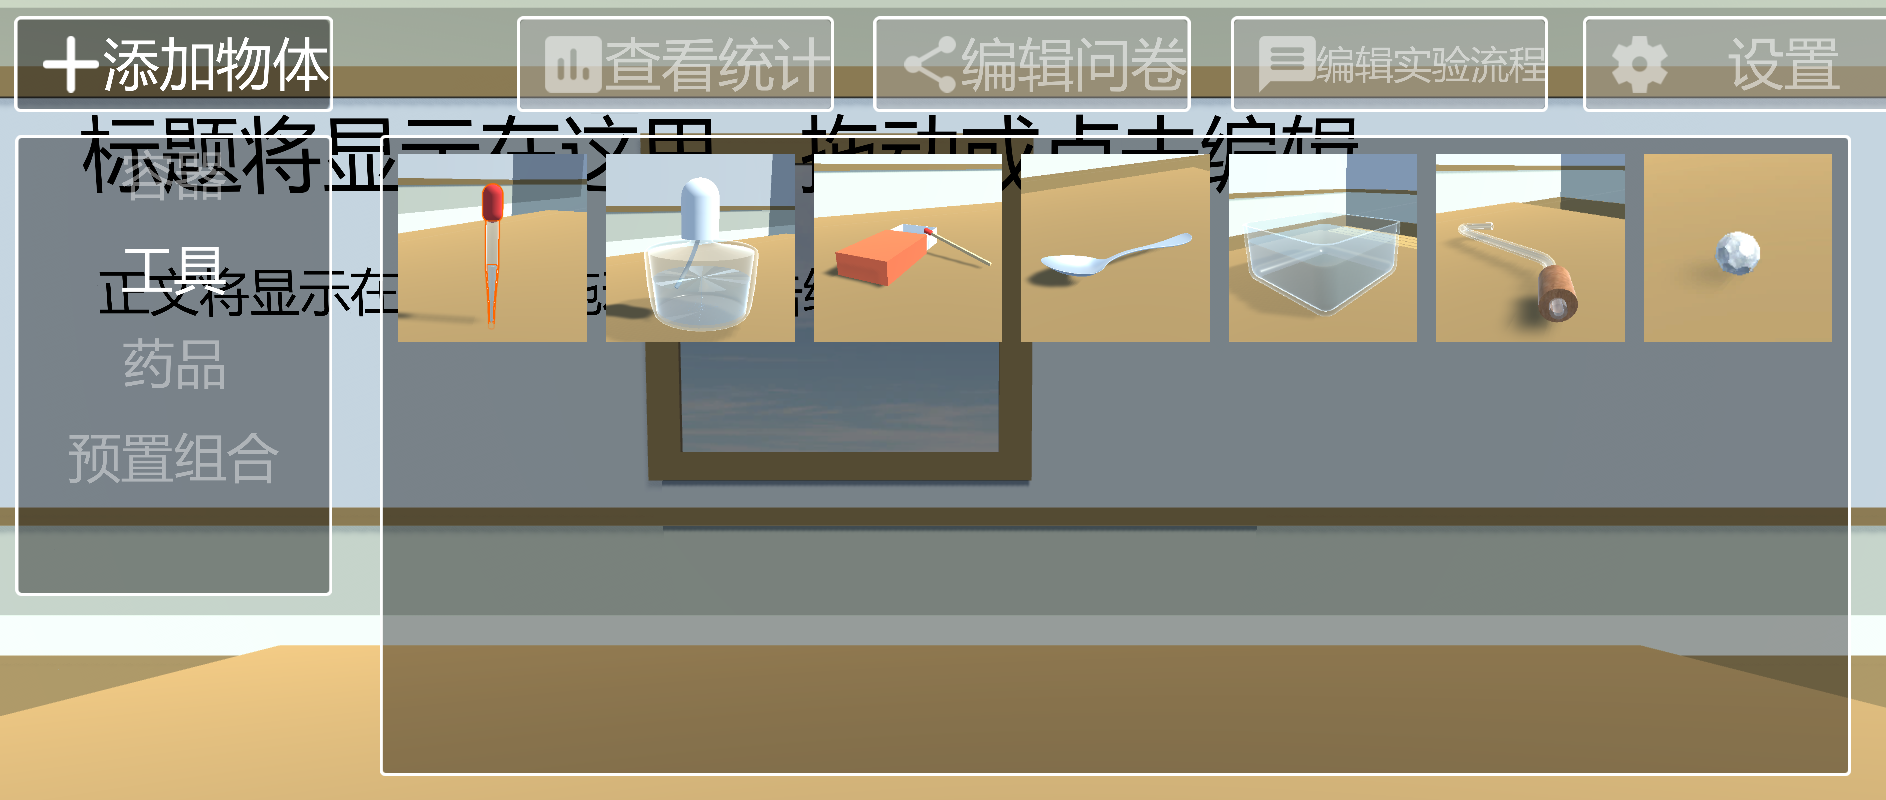
\includegraphics[width=12cm]{figure/addObj.png}
  \bicaption[添加物体用户接口截图]
    {添加物体用户接口截图}
    {The Screen-shot of Adding Object UI}
 \label{fig:gm}
\end{figure}

	创建好的物体通过控制器Lab\_Controller进行控制。Lab\_Controller会在用户触发点击事件时,从相机向屏幕点击位置发出一条射线,并获取射线碰撞的第一个物体。同时,控制器会在每一帧计算距离用户点击时刻的时长,如果在到达一定的阈值之前检测用户松开鼠标,则触发单击对应的事件。如果超时,则会判断用户触发拖动事件。

	如果是单击事件,首先判断接触到的是否是可以编辑的容器,判断的方式是该物体是否具有container类,该类用于保存物体包含的物质的种类和量。如果有,则显示编辑物质的菜单(Substance Menu)。下拉框会在初始化的时候获取所有支持的物质,并且修改选项。为了保证物质的量为浮点数,需要对输入框的格式进行设置。完成编辑后,控制器会将用户输入赋值到该物体的container对象中。如果没有,则无效果。
	
\begin{figure}[!htp]
  \centering
  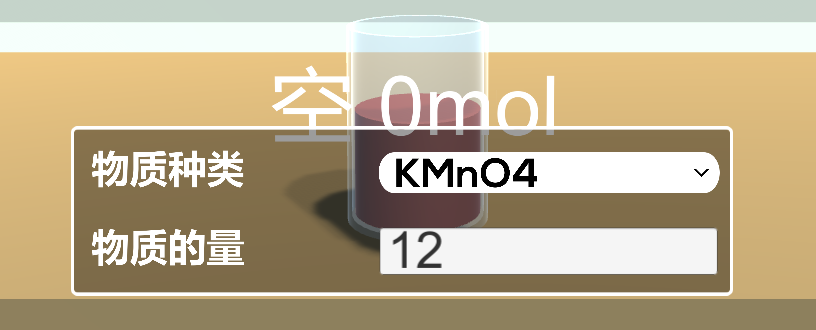
\includegraphics[width=12cm]{figure/subs.png}
  \bicaption[编辑物体种类用户接口截图]
    {编辑物体种类用户接口截图}
    {The Screen-shot of Editing Object UI}
 \label{fig:subs}
\end{figure}

编辑好的物体会将物质信息显示在模型外,效果见图\ref{fig:subs}和\ref{fig:substi}。显示的文字通过3D Text实现,会在修改之后触发相应的函数修改其text mesh的内容。

如果是拖动事件,依然首先判断物体是否是可以移动的物体,所有添加的物体都是可以移动的,他们使用Object的标签进行标记。判断的目的是避免拖动桌子、墙壁等静态物体。之后会在每一帧由相机向鼠标位置发出射线,将当前拖动的物体放置在射线和碰撞体的交点上。此时需要先去除拖动物体的碰撞体,否则物体会沿着射线方向一直向相机移动。当用户松手的时候,物体就会停留在最后移动的位置,并且恢复物体的碰撞体保证可以进行下一次移动。

由于一些实验中往往需要流程化的实验步骤,例如产生气体之后通入水槽等,需要气体发生装置和收集装置相对位置固定,因此添加了UI\_Anchor进行引导。UI\_Anchor是与桌面平行的平面碰撞体,当上述的交点接触到锚点(anchor)时(同样使用tag进行标记),会在锚点中心生成一个当前拖动物体的复制,并且修改它的材质为半透明单色,并把该物体的指针赋给UI\_Anchor中的对应变量。如果此时用户松开鼠标,则拖动中的物体就会代替复制,被固定在锚点上。当用户需要将物体从锚点移开的时候,则会制造先出复制,直到点击位置离开锚点范围之后才删除复制,在这过程中如果用户松开鼠标,则物体会返回锚点处。
	
\begin{figure}[!htp]
  \centering
  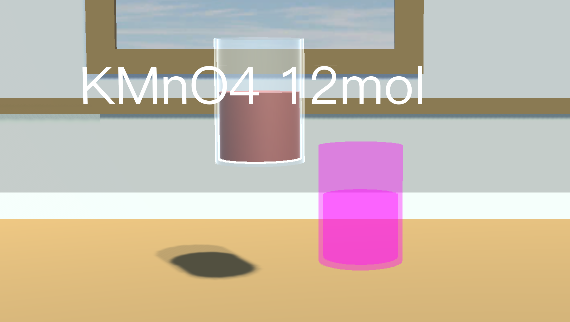
\includegraphics[width=8cm]{figure/substi.png}
  \bicaption[锚点物体复制效果图]
    {锚点物体复制效果图}
    {The Effects of Objects Substitution on Anchor}
 \label{fig:substi}
\end{figure}

场景中有多个平行锚点,它们都在同一个实验桌上,由UI\_Table控制。UI\_Table会储存桌子上的锚点的物体信息,并且在鼠标移入、移出锚点,即真正添加和删除物体的时候,根据所有锚点的位置和占用情况,对其余物体进行移动操作。如果在添加的时候发现所有的锚点都被占用,则不会创建新的复制,物体也不能被移入锚点。

基于上述机制,物体在创建的时候会优先创建在锚点上。只有当物体太多、锚点都被占用的时候,才会被创建在桌面上的其他位置。综上所述,实现了物体的创建、移动、内容编辑的功能。


\subsection{提示信息编辑}
实验过程中需要显示实验名称,并且提示用户实验步骤,用户可以通过编著系统修改提示信息的位置、大小、颜色等属性。

\begin{figure}[!htp]
  \centering
  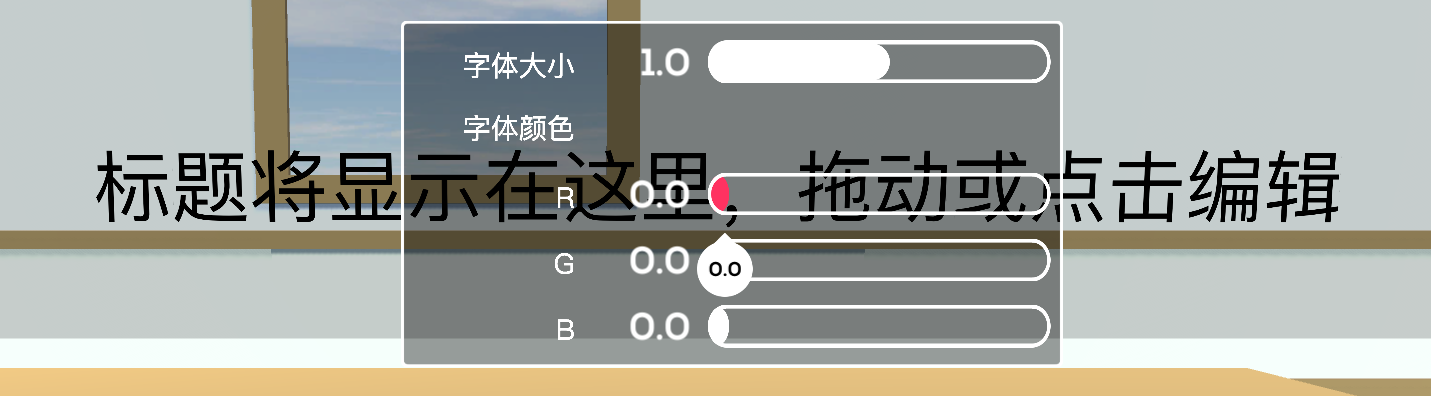
\includegraphics[width=12cm]{figure/text.png}
  \bicaption[编辑提示文字外观用户接口截图]
    {编辑提示文字外观用户接口截图}
    {The Screen-shot of Editing Hints Appearance UI}
 \label{fig:gm}
\end{figure}

用户可以编辑提示文字的显示方式。在lab controller获取到点击事件之后,如果点击的物体标签为text,则会首先获得物体中的text对象,用其中的属性值,包括字体的颜色、大小,初始化字体编辑的菜单控件的值,然后显示该菜单。用户在编辑之后,相应的文字就会被修改并显示了,编辑完成后,还会修改字体的text对象的变量值,保证下一次操作的正确性。

当用户触发拖动事件,则按照与移动物体相似的逻辑移动字体,只不过在移动物体的时候如果点击位置不在字体可显示范围之内,文字就不会再发生移动。由于这些文字需要在三维场景中移动,因此也使用了3D Text。但是3D Text默认情况下会永远显示在最前面,如果需要其具有深度关系,需要修改使用的着色器。起初,本系统自定义了新的着色器,但是,修改之后的着色器只能通过修改材质中的颜色参数才能修改颜色,修改text mesh的颜色是无效的,这在一些使用场景下(如WebGL)下是不被支持的。此外,该着色器会使文字在一定位置显示特殊的反射,影响观感。最简单有效的方法是将3D text的着色器修改为一般的2D字体的着色器,然后使用中文字体。

\subsection{实验流程编辑}
用户可以通过编著系统,编辑用户在进行实验时参考的提示信息内容。

\begin{figure}[!htp]
  \centering
  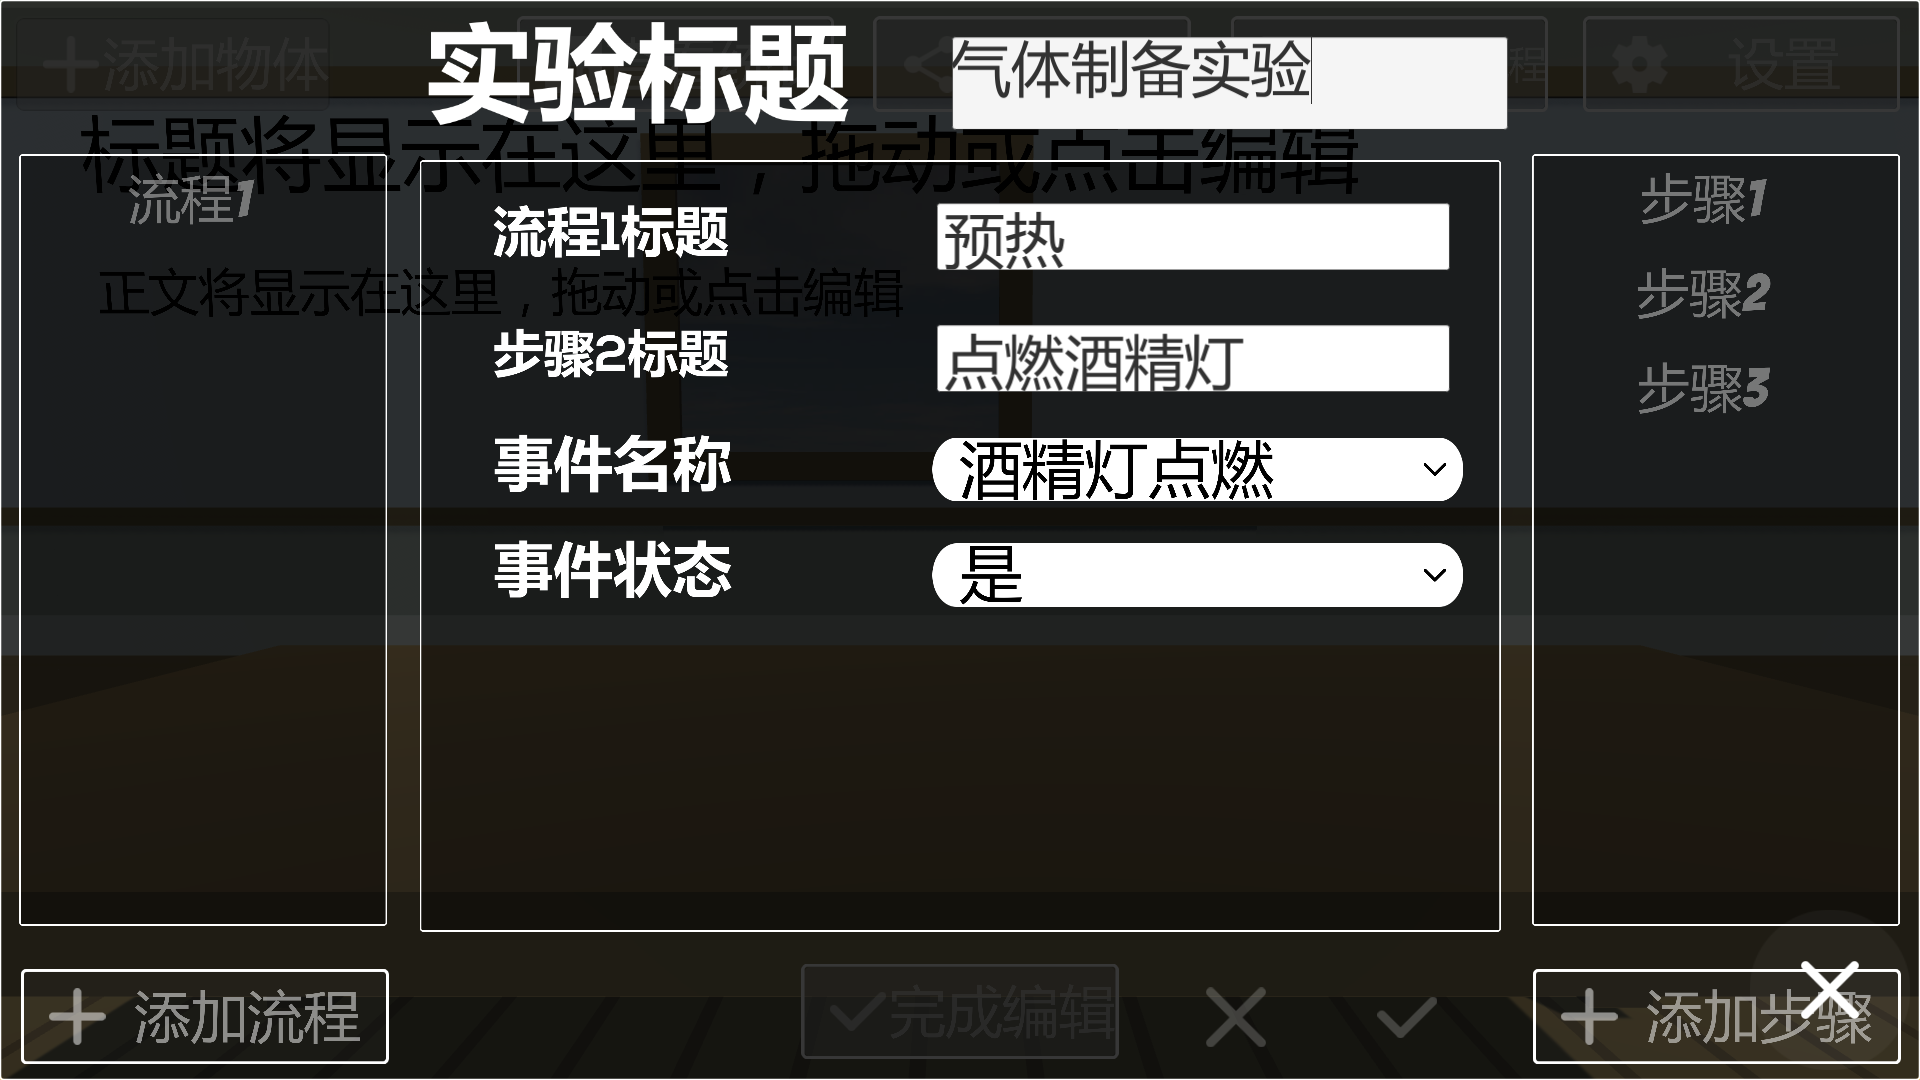
\includegraphics[width=12cm]{figure/step.png}
  \bicaption[编辑实验流程用户接口截图]
    {编辑实验流程用户接口截图}
    {The Screen-shot of Editing Experiment Procedure UI}
 \label{fig:gm}
\end{figure}

当用户选择实验流程编辑的时候,会显示对应的菜单。用户可以添加流程,流程由预制体构成,添加的流程将会追加在显示流程的滑动框(scroll content)的子对象中,并且自动按照vertical layout进行排列。点击一个创建的流程之后可以为它添加对应的步骤,步骤使用同样的预制体实现,使用布尔值进行区分。添加的步骤会追加在显示步骤的滑动框中。流程、步骤都可以通过输入框修改名称,步骤还需要设置对应的操作事件,可用的操作事件会在菜单初始化的时候向游戏管理器发出请求获取,并且通过下拉框供用户选择。关于步骤、流程的上述属性都会在发生修改之后,保存在各自的step对象中。

编辑信息由UI\_Step进行控制。他保存了一个记录所有流程的指针数组,以及记录每个流程对应步骤的二维指针数组。UI\_Step还记录了当前的流程和步骤序号,当用户切换步骤的时候,会读取当前的step中的信息,并且把对应数据显示在控件上。当用户切换流程的时候,会从二维指针数组中激活对应的步骤,而将当前显示的所有步骤隐去。


\subsection{编辑已有实验}
用户可以保存已经编辑的实验,在下一次使用的时候继续编辑。负责该功能的是UI\_Edit。他会在用户保存编辑内容的时候,将场景数据保存在游戏管理器的experiment setup对象中,其结构见图\ref{fig:uml},并且通过网络发送数据,保存在数据库。其中场景的编辑数据通过对应的编辑菜单获得,场景中的提示信息数据通过场景中的两个文字对象的相关属性获得。所有的物体创建后都会成为object list的子对象,遍历object list可以获得所有创建物体的相关属性。而实验流程则通过保存在UI\_Step中的两个列表获得。

将上述变量保存之后,在编辑已有场景的时候,场景会在初始化的时候从游戏管理器读取该对象,将所有属性还原。其中场景的还原,包括将还原的数据作用于场景中的对象上,并且修改场景编辑菜单控件的初始值。提示文字按照数据修改相应的颜色、位置等数值。物体的还原需要按照物体的名字、物质的量等信息,重新初始化游戏对象,仍然添加在object list下。步骤的还原需要还原出所有的流程、步骤按键,并且放置在对应的滑动框的子对象下,还需要还原UI\_Step中的记录所有流程的指针数组,和记录每个流程下的步骤的二维指针数组。之后场景的还原就完成了,用户可以在此基础上继续编辑实验。

\section{编著系统结果与分析}
系统在PC端和安卓手机端都进行了安装,两者都可以完成预期的工作。

在使用手机应用进行实验编著时,用户可以顺利完成点击、拖动等操作,实现预期需求,例如图\ref{fig:authorRes}中展示的,实验器具和药品的添加和编辑,物体移动,实验环境的编辑,实验流程的编辑等。所有的交互方式与PC端保持一致,只需要用手指触摸代替鼠标点击。此外,通过用户试用反馈来看,在物体的创建、编辑等部分可以很快操作,但是流程编辑的部分则有些复杂。

\begin{figure}[!htp]
  \centering
  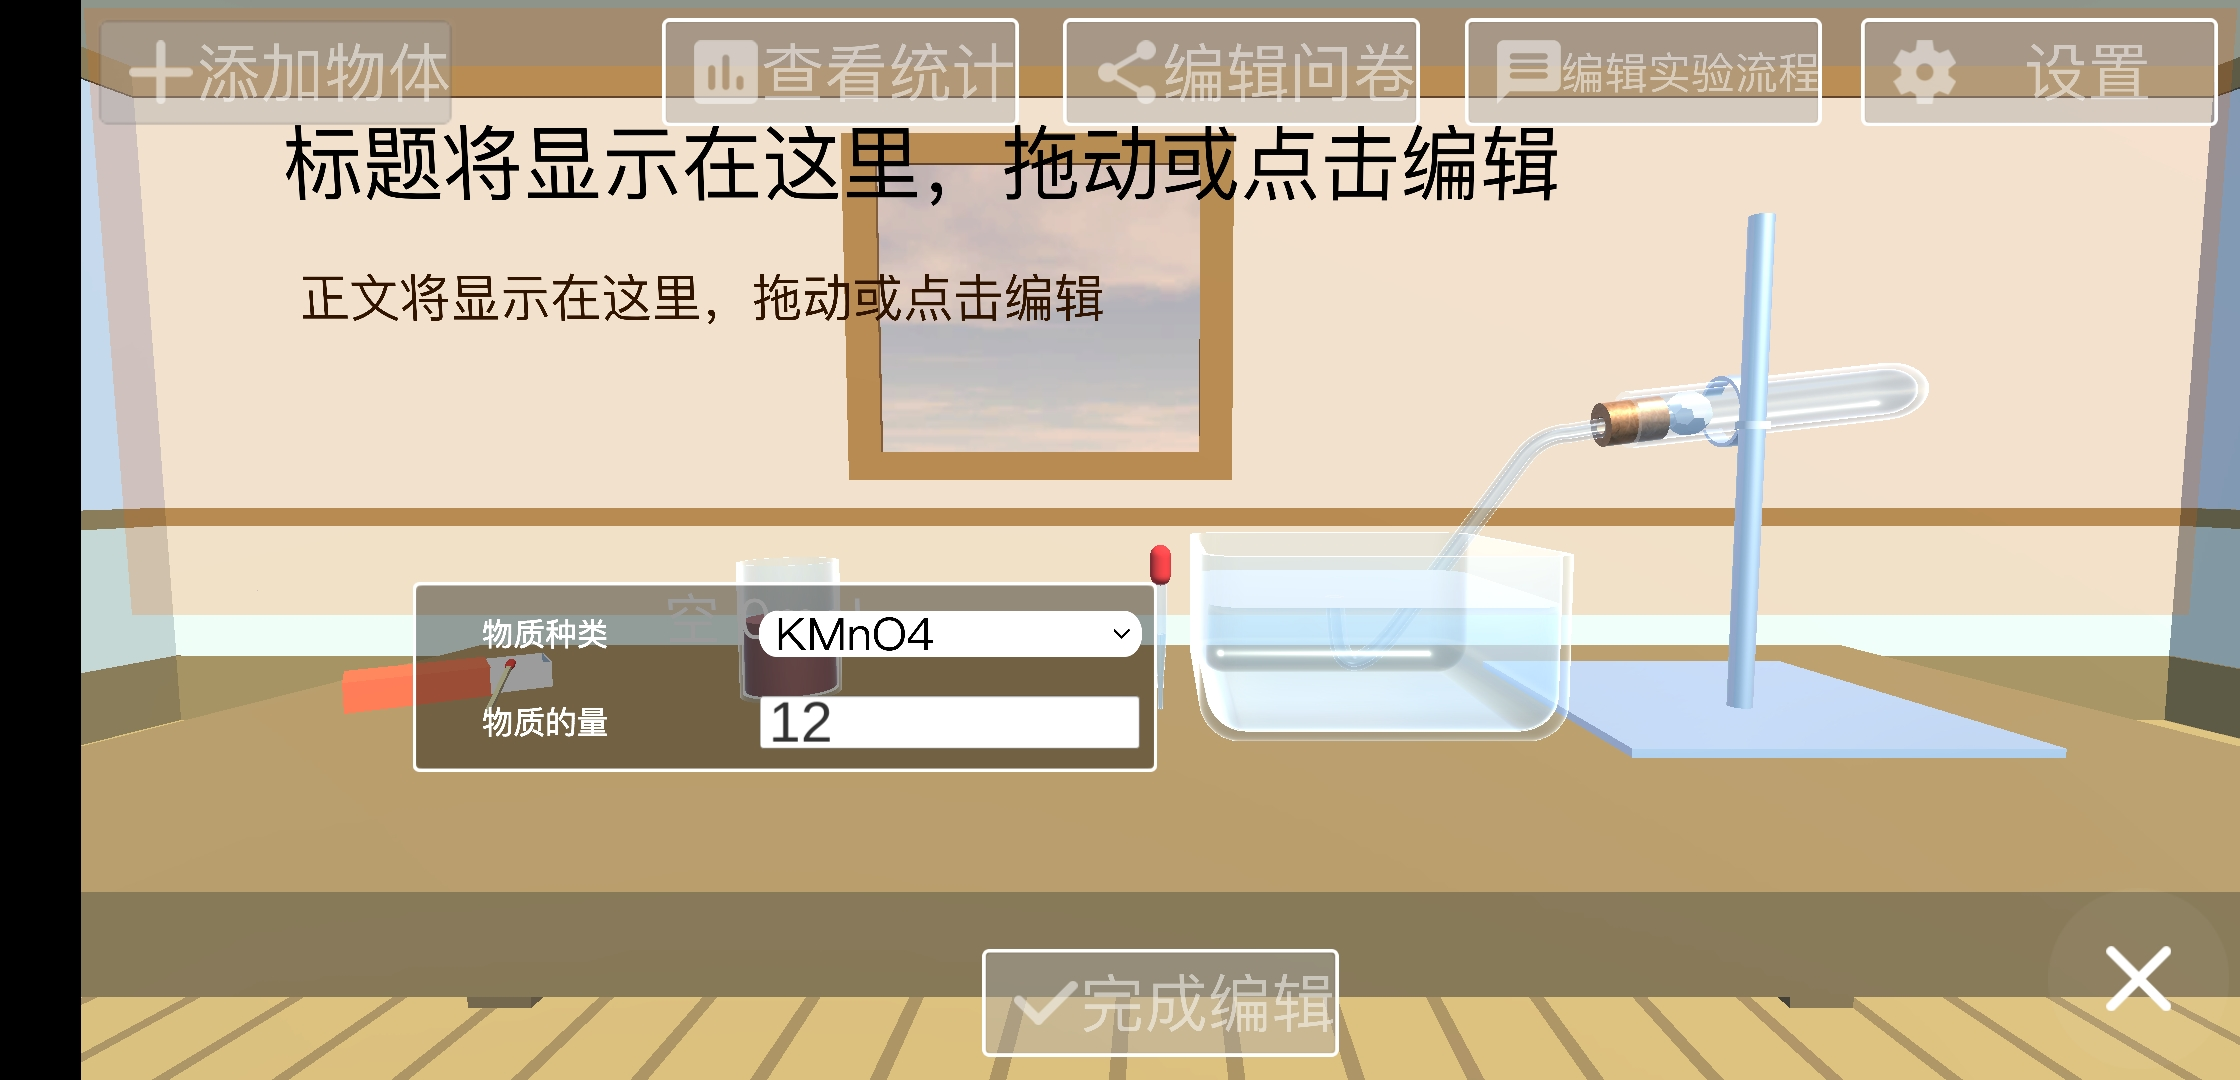
\includegraphics[width=6cm]{figure/objRes.jpg}
  \hspace{1cm}
    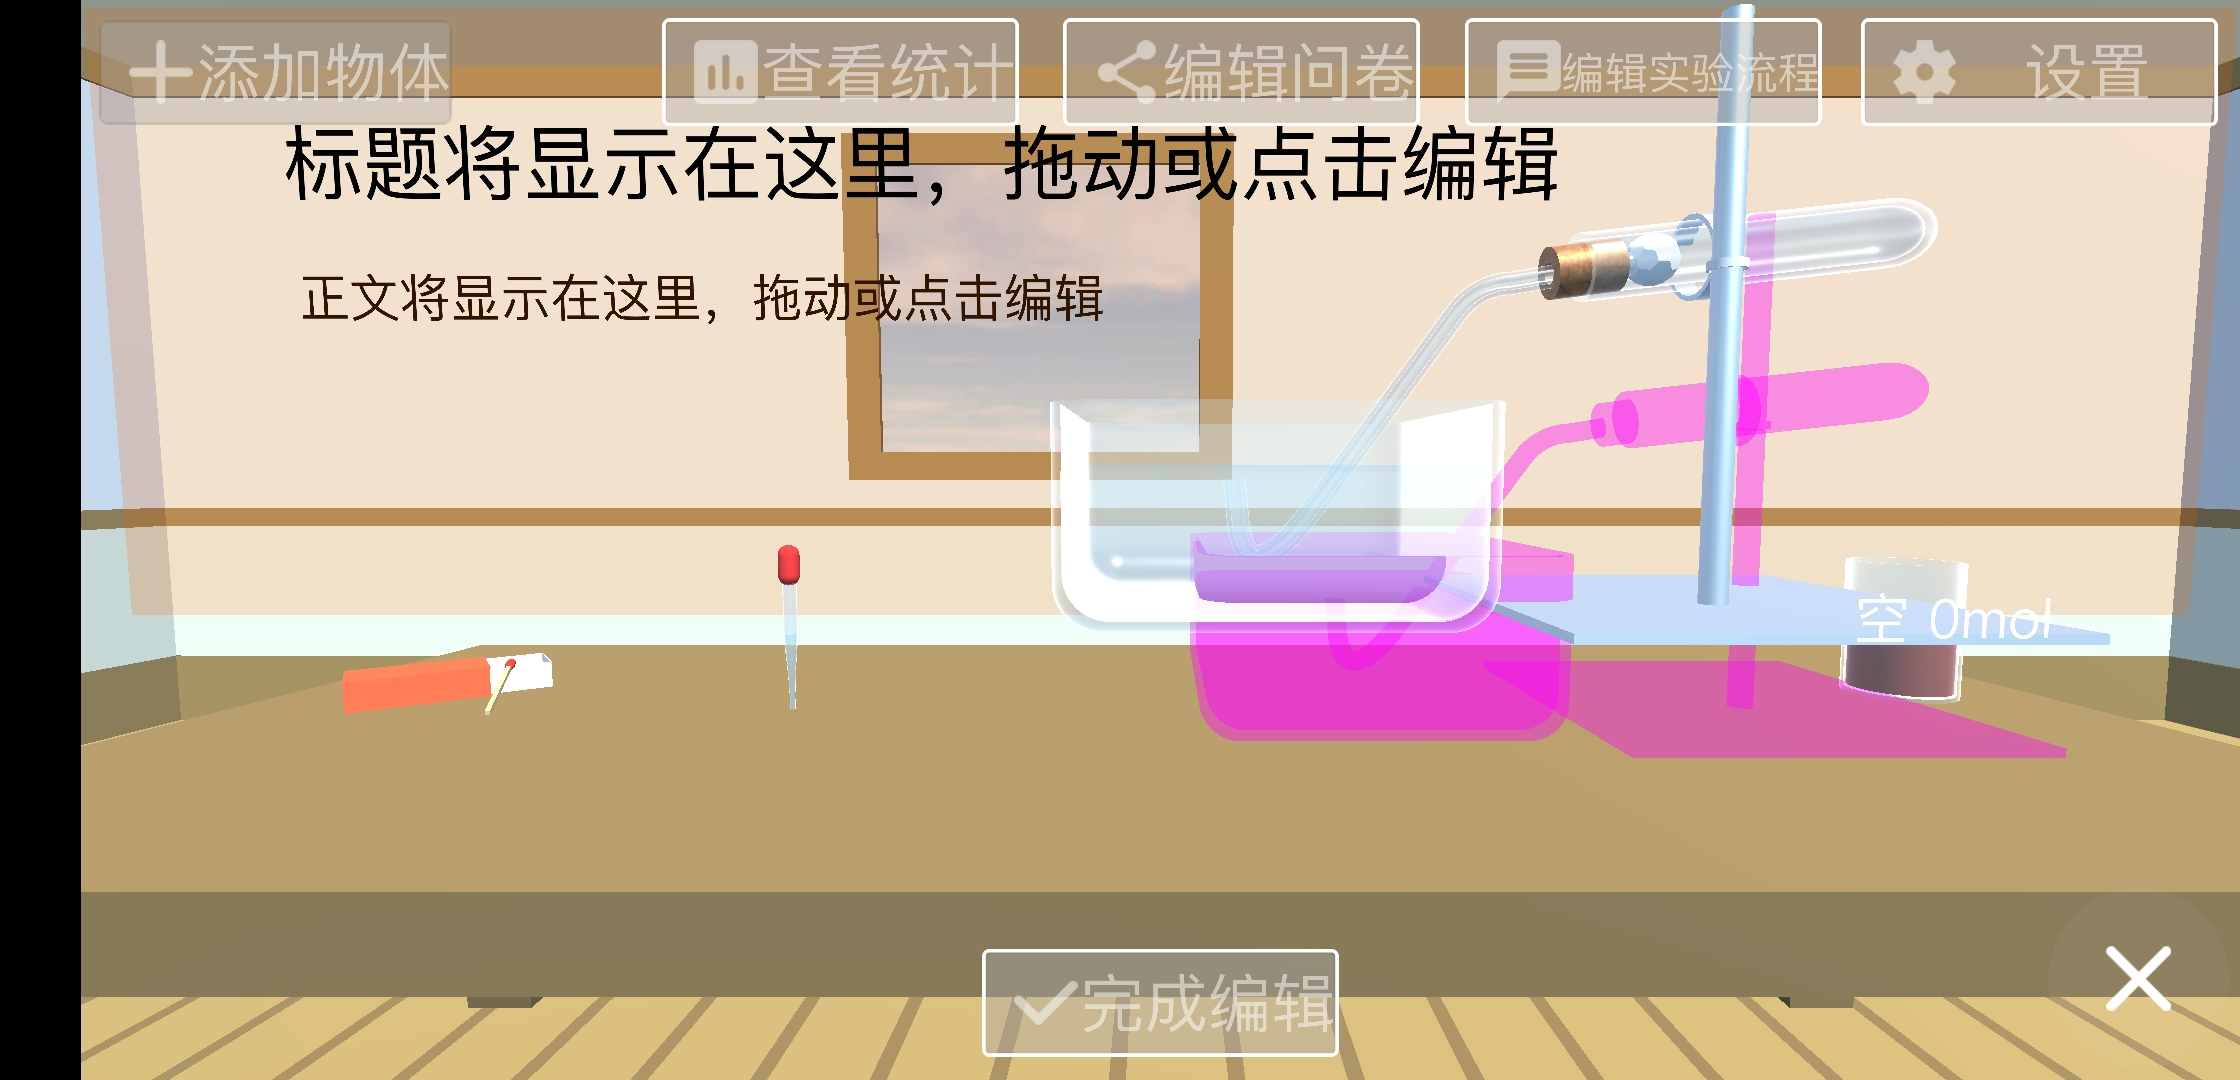
\includegraphics[width=6cm]{figure/movingRes.jpg}
    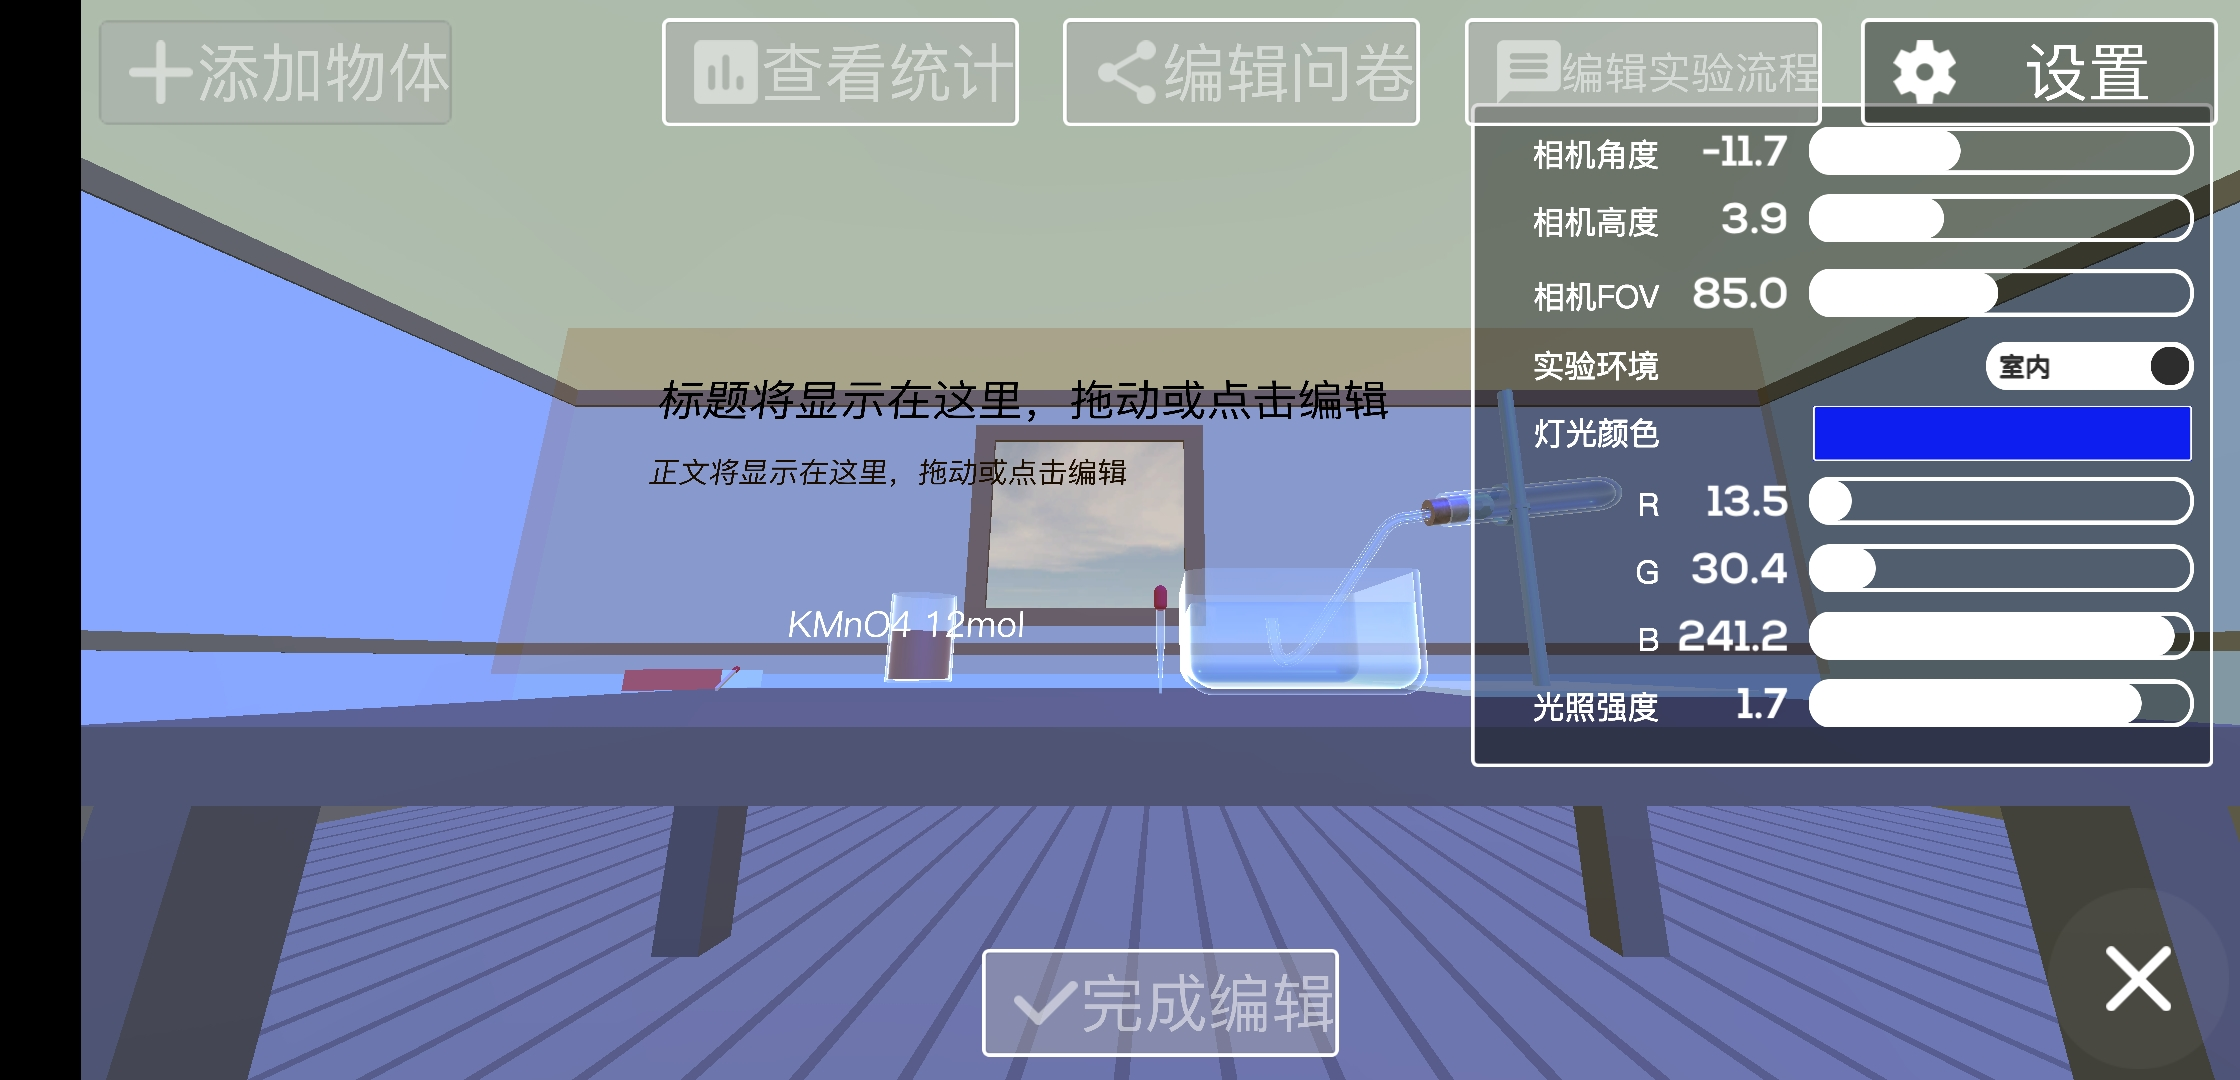
\includegraphics[width=6cm]{figure/envirRes.jpg}
  \hspace{1cm}
  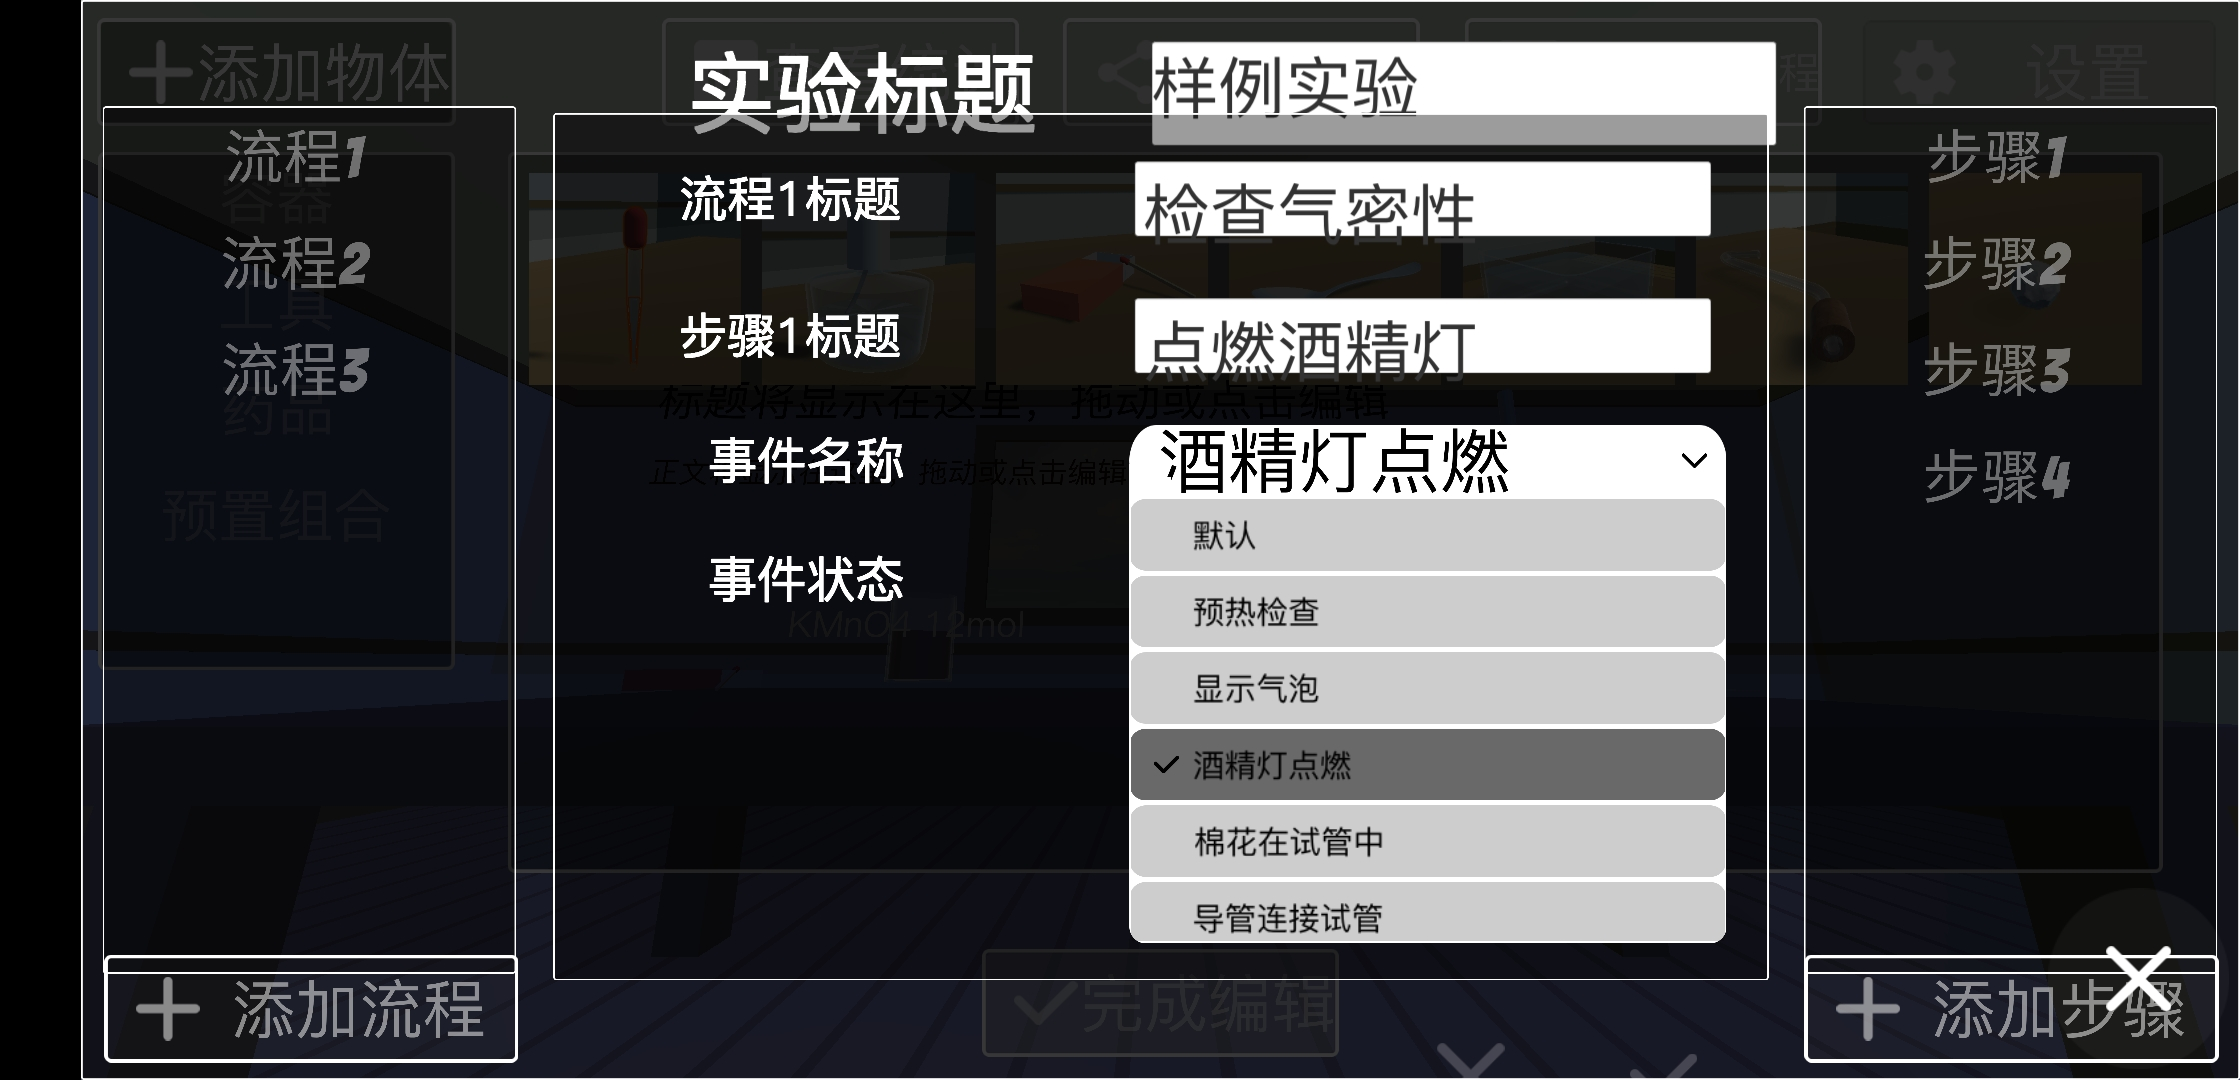
\includegraphics[width=6cm]{figure/procedureRes.jpg}
  \bicaption[手机端编著系统截图]
    {手机端编著系统截图}
    {The Screen-shots of Authoring System on Mobile Device}
 \label{fig:authorRes}
\end{figure}

系统目前支持了工具、容器、药品、预置组合四大类物品,包括酒精灯、集气瓶、火柴、水槽、烧杯等高中化学实验需要的器材,以及铁、高锰酸钾、稀盐酸等高中化学实验常用药品。通过组合所有支持的器材和药品,用户可以编辑出完整的高锰酸钾制氧气的实验。

\begin{figure}[!htp]
  \centering
  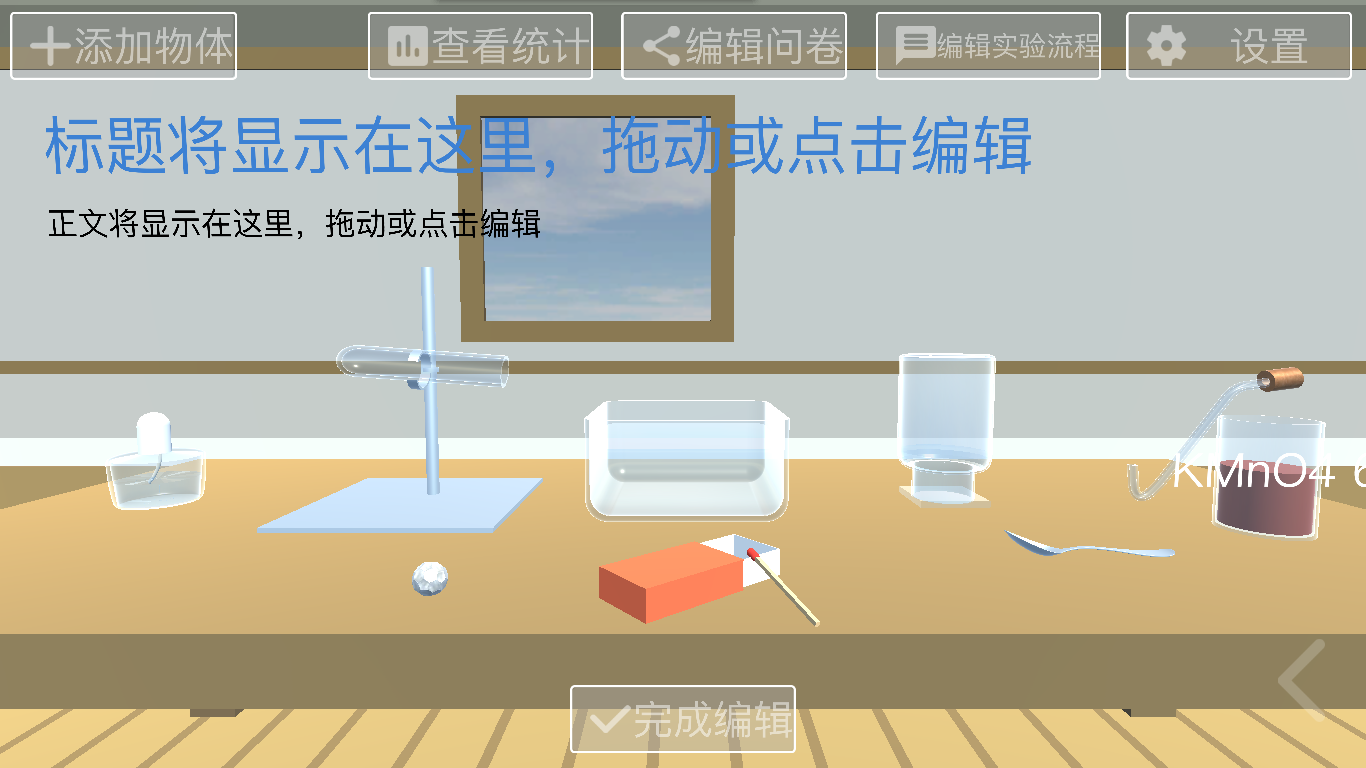
\includegraphics[width=12cm]{figure/Kmno4res.png}
  \bicaption[编著高锰酸钾制氧气实验截图]
    {编著高锰酸钾制氧气实验截图}
    {The Screen-shot of Authoring the Oxygen Production Experiment with $KMnO_4$}
 \label{fig:authorRes}
\end{figure}

\section{本章小结}
本章从需求分析、系统设计与实现、结果分析的角度详细介绍了为教育者提供的编著平台是如何完成的。从需求分析角度,我们对用户的使用习惯、功能需求、硬件条件进行分析,总结出编著系统应当具备的功能。之后完成系统设计。系统分为用户接口、引擎、持久化对象三层,并根据设计完成了项目各功能的实现。最后,我们对于编著系统的功能进行汇总并且分析了使用感受。